\subsection{Boosting Signal Power: The Magic of Phased Driven Elements!}

\begin{tcolorbox}[colback=gray!10, colframe=black, title=E9E11] What is the purpose of using multiple driven elements connected through phasing lines?

\begin{enumerate}[label=(\Alph*)]
    \item \textbf{To control the antenna’s radiation pattern}
    \item To prevent harmonic radiation from the transmitter
    \item To allow single-band antennas to operate on other bands
    \item To create a low-angle radiation pattern
\end{enumerate} \end{tcolorbox}

In radio communication, antennas are critical components that determine how signals are transmitted and received. The use of multiple driven elements, particularly when connected through phasing lines, is a technique employed primarily to manipulate the radiation pattern of an antenna system.

The correct answer to the question is option A: To control the antenna’s radiation pattern. 

The ability to control radiation patterns is instrumental for various communication applications, as it allows for focusing energy in desired directions and minimizing interference. This is achieved through the design and configuration of the antenna array. 

The concept of phasing lines is integral to this process. Phasing lines are lengths of transmission line that connect multiple antennas. By adjusting the lengths of these lines and the relative phase of the signals supplied to each driven element, it is possible to steer the main lobe of the radiation pattern, as well as control side lobes, thus optimizing communication efficiency and range.

To understand this further, consider the following:
1. \textbf{Radiation Pattern:}: This visualizes the distribution of radio waves in space as emitted by the antenna. The main lobe indicates the direction of strongest radiation, while side lobes can indicate potential interference.
2. \textbf{Phasing:}: This involves coordinating the timing of the signals sent to each antenna element. Proper phasing can reinforce or cancel signals in different directions.
  
For instance, if you desire a high-gain directional antenna system, you could use two elements where one is fed with a signal that is phase-delayed. This delay can be achieved using varying lengths of transmission lines, effectively manipulating the relative phases of the signals at the driven elements.

To illustrate the concept, we can use TikZ to draw a simplified diagram of a two-element linear array antenna with connected phasing lines: 

\begin{center}
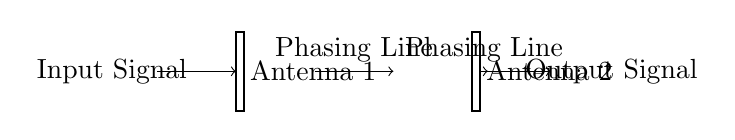
\begin{tikzpicture}
    % Antenna Elements
    \draw[thick] (0,0) rectangle (0.1,1) node[midway, right] {Antenna 1};
    \draw[thick] (3,0) rectangle (3.1,1) node[midway, right] {Antenna 2};
    
    % Phase Lines
    \draw[->] (1,0.5) -- (2,0.5) node[midway, above] {Phasing Line};
    \draw[->] (3.1,0.5) -- (3.2,0.5) node[midway, above] {Phasing Line};

    % Input Lines
    \draw[->] (-1,0.5) -- (0,0.5) node[midway, left] {Input Signal};
    \draw[->] (3.1,0.5) -- (4,0.5) node[midway, right] {Output Signal};
\end{tikzpicture}
\end{center}

In summary, employing multiple driven elements with appropriate phasing connections is key to enhancing antenna function by controlling radiation patterns, which can dramatically affect the efficacy of communications.